\chapter{ Констукторский раздел}
\label{cha:design}
    В данном разделе будут рассмотрены схемы алгоритмов, требования к функциональности ПО,
    опредены способы тестирования и подсчитана сложность алгоритмов.
    
    \section{Разработка алгоритмов}
        Ниже будут представлены схемы алгоритмов сортировки: \begin{enumerate}
            \item алгоритм сортировки пузырьком с флагом (рисунок \ref{schema:sort:bubble});
            \item алгоритм сортировки вставками  (рисунок \ref{schema:sort:insertion});
            \item алгоритм сортировки выбором (рисунок \ref{schema:sort:selection}).
        \end{enumerate}

    \begin{figure}[h!]
        \centering
            \includegraphics[scale=0.9]{schema_bubble.pdf}
            \caption{Схема алгоритма сортировки пузырьком с флагом}
            \label{schema:sort:bubble}
    \end{figure}

    \begin{figure}[h!]
        \centering
            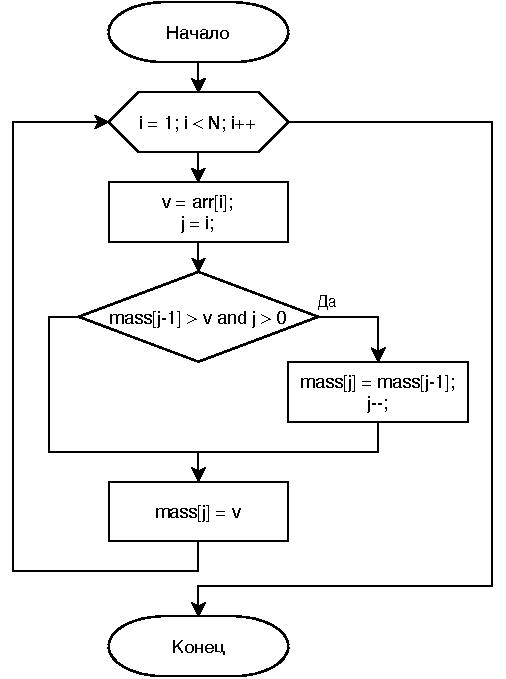
\includegraphics[scale=0.9]{schema_insertion.pdf}
            \caption{Схема алгоритма сортировки вставками}
            \label{schema:sort:insertion}
    \end{figure}

    \begin{figure}[h!]
        \centering
            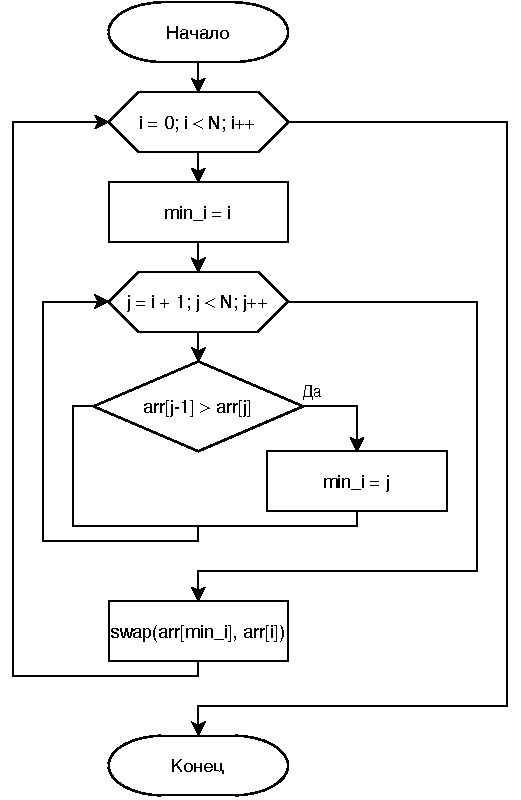
\includegraphics[scale=0.9]{schema_selection.pdf}
            \caption{Схема алгоритма сортировки выбором}
            \label{schema:sort:selection}
    \end{figure}

\section{Оценка трудоёмкости алгоритмов сортировки}
        Во всех теоритических оценках трудоёмкости
        алгоритмов сортировки предполагается, что
        трудоёмкость сравнения $ f_{cmp} = 2 $.

        \subsection{Алгоритм сортировки пузырьком c флагом}
            Найдём трудоёмкость алгоритм сортировки пузырьком c флагом.
            
            Лучший случай -- массив отсортирован; 
            не произошло ни одного обмена за 1 проход,
            следовательно выходим из цикла, тогда
            трудоёмкость определяется по следующей формуле:

            \begin{equation}
                f = 1 + 2 + (2 + 1 + 2 + (N - 1) (2 + 3) + 2) = 5N + 8= O(N)
            \end{equation}

            Худший случай -- массив отсортирован в обратном порядке; 
            На каждой итерации происходил обмен, тогда
            трудоёмкость определяется по следующей формуле:

            \begin{equation}
                f = 1 + 2 + \sum_{i=1}^N (2 + 1 + 2 + (N - i)(2 + 4) + 1) = 3N^2 + 3N + 3 = O(N^2)
            \end{equation}

        \subsection{Алгоритм сортировки вставками}
            Найдём трудоёмкость алгоритма сортировки вставками.
                
            Лучший случай -- массив отсортирован. 
            При этом все внутренние циклы состоят всего из одной итерации, тогда
            трудоёмкость определяется по следующей формуле:

            \begin{equation}
                f = 1 + 2 + (N-1)(2 + 3 + 2 + 2 + 1) = 10N - 7 = O(N)
            \end{equation}

            Худший случай -- массив отсортирован в обратном порядке. 
            Каждый новый элемент сравнивается со всеми в отсортированной последовательности.
            Все внутренние циклы будут состоять из j итераций, тогда
            трудоёмкость определяется по следующей формуле:

            \begin{equation}
                f = 1 + 2 + (N-1)(2 + 3 + \sum_{i=1}^{N-1} (2 + 2 + 1 + 4 + 1) + 1) = 10N^2 - 14N + 7 = O(N^2)
            \end{equation}

        \subsection{Алгоритм сортировки выбором}
            Трудоёмкость сортировки выбором в худшем и лучшем случаях совпадает
            и оценивается как $ O(N^2) $.       


    \section{Требования к функциональности ПО}
        В данной работе требуется обеспечить следующую минимальную функциональность консольного приложения:
        \begin{enumerate}
            \item предоставить возможность ввода массива, на выходе пользователь должен получить результат сортировки массива, произведенной тремя алгоритмами;
            \item обеспечить вывод замеров времени работы каждого из алгоритмов в худшем, лучшем и произвольном случаях.
        \end{enumerate}

    \section{Методы тестирования}
    Тестирование ПО будет проводиться методом чёрного ящика. Необходимо проверить работу системы 
    на тривиальных случаях: список является пустым или содержит один элемент,
    и несколько нетривальных случаев: список отсортирован по возрастанию / по убыванию, случайный список.

\newpage